% \revise{
\chapter{LeapFi: A Learning-based Application-oriented IEEE 802.11 System Channel Access Framework}
\label{ch3_after}

%=================================================================================================%
%=================================================================================================%

Reinforcement learning (RL) for radio resource management has attracted considerable attention, due to its promising ability to deal with unknown system statistics while significantly reducing the computational complexity compared to conventional model-based reinforcement learning approaches.
For example, it is prohibitively expensive to acquire co-channel interference caused by other traffics in unlicensed frequency bands, such as those used by the IEEE 802.11 system.
% it is also difficult to retrieve sufficient media access control (MAC) layer and physical (PHY) layer states from commercial Wi-Fi adapters.
Hence, the communication resource scheduling of a Wi-Fi network is challenging.
In this Chapter, we would like to leverage the state-of-the-art reinforcement learning techniques to facilitate the coordination of the Wi-Fi network transmission and to address the aforementioned practical constraints, so that the quality-of-service (QoS) of the heterogeneous applications is optimized.
% Moreover, the RL technique has also great potential to optimize a wireless system even without accurate or complete observation of the system state, which might happen in practical implementations.

There have been a significant amount of works optimizing the throughput~\cite{zhang2020drlthoughput,chu2018reinforcement,xu2020buffer}, delay~\cite{zhang2020delay} or age-of-information (AoI)~\cite{abd2020reinforcement,wu2022aoi,9839316} of wireless networks via the method of RL.
All these works assumed full knowledge of the system state in algorithm design, which could be applied on the systems where the global system state could be collected at a centralized controller. On the other hand, RL was also utilized to optimize the performance of wireless systems with distributive transmission scheduling, e.g., Wi-Fi systems. For instance, an adaptive channel contention mechanism was proposed for Wi-Fi systems in~\cite{kumar2021adaptive}, where a local RL agent is deployed at each user equipment (UE). The local agents adjust the minimum contention window (MCW) size according to the global statistics of successful channel contention such that the transmission fairness among the agents can be ensured.
% Enhancing Wi-Fi multiple access performance with federated deep reinforcement learning
Instead of global statistics, a distributive RL algorithm with the assistance of federated learning was proposed in~\cite{zhang2020enhancing} to adapt the channel contention according to the local channel state, such that the local throughput was optimized. Moreover, a deep multi-agent RL technique based on the QMIX algorithm~\cite{rashid2020monotonic} was proposed in~\cite{guo2022multi} to improve network throughput while maintaining user fairness. In this work, the channel contention decision was made according to the history of the last transmission duration. In order to resolve the collision issue of the distributive channel access, deep RL algorithms were proposed in~\cite{ali2018deep,ali2019q} to determine the timing of doubling the contention window based on the estimated collision probability.
% An Experience Driven Design for IEEE 802.11ac Rate Adaptation based on Reinforcement Learning
In addition to the adaptive channel contention, a double deep Q-network (DDQN)~\cite{van2016deep} based rate adaptation algorithm was proposed in~\cite{chen2021experience} to improve network throughput, where the agent learned the optimal transmission rate based on the modulation and coding scheme (MCS) and frame loss rate.

Most of the above literature assumed knowledge of the PHY-layer and MAC-layer system states. The RL techniques were exploited to tackle the unknown state transition probabilities or seek good scheduling policies from their enormous policy space. However, it might be challenging to obtain the knowledge of the PHY-layer and MAC-layer states in the controller design of a practical Wi-Fi network. Although there are some testbeds extracting the PHY-layer information from the adapter, e.g.,\cite{chen2021experience}, these methods would degrade the transmission performance due to hardware limitations and might not be generalized to most Wi-Fi adapters. Moreover, the absent knowledge on co-channel interference and the vendor-dependent implementation of Wi-Fi adapters would also raise challenge on the optimization of scheduling policies. 

In this Chapter, we would like to shed some light on the RL-based scheduling design for practical Wi-Fi systems suffering from unknown co-channel interference. Specifically, a learning-based framework for the application-layer QoS Optimization of Wi-Fi networks, namely {\algName}, is proposed for the scheduling of delay-sensitive communication tasks and throughput-hungry file delivery tasks. In {\algName}, a controller periodically collects the past scheduling parameters and average QoS observations of all the application-layer tasks, determines rate limitation and contention window size for all the transmitters, such that the total throughput of file delivery tasks is maximized and the latency requirements of delay-sensitive tasks are ensured. Because the relationship between the application-layer QoS and the transmission scheduling parameters is unknown, a novel Q-network design is proposed, which maps the historical scheduling parameters and QoS observations to the current scheduling action. Moreover, an imitation learning method is introduced to improve the training efficiency of the Q-network. It is shown by the experiments that the proposed framework can adapt to the variation of task number, interference traffic and link quality, and significantly outperforms the conventional EDCA mechanism.

\section{System Model}
In this section, the deployment scenario of the proposed {\algName} system is first elaborated, followed by the models of transmission and scheduling.

\subsection{Deployment Scenario}
\label{sec:Deployment Scenario}

The proposed {\algName} system is deployed in a Wi-Fi network (i.e., an extended service set, ESS) with multiple connected access points (APs) and user equipments (UEs) working on the same channel. Denote the number of the devices, including the APs and UEs, in the Wi-Fi network as $U$, the set of these devices as
\begin{equation}
    \devSet =\{u_{i}|{i}=\iterDeviceSet\},
\end{equation}
and the communication link from the $i$-th device to the $j$-th one as the {$(i,j)$}-th link ($\forall u_{i}, u_{j} \in \devSet$). The communication links can be from UE to AP, from AP to UE, or between UEs (i.e., Wi-Fi Direct~\cite{alliance2009wi}). We define $\linkset$ as the set of all communication links in the system and $\linkset_{i} $ as the set of communication links from the $u_{i}$-th device. As a remark, one UE could be with both the infrastructure and Wi-Fi Direct modes. Thus, it could simultaneously maintain the communication links to the AP and other UEs, where the transmission of the infrastructure and Wi-Fi Direct modes is separated in the time domain.

The data traffics raised by the applications of UEs in $\devSet$ are referred to as communication tasks in this Chapter. For example, the application projecting the screen of a mobile phone to a laptop via Wi-Fi Direct will raise a {\it delay-sensitive task}, e.g., Miracast~\cite{WiFiDisplay2011}, where an application-layer packet (i.e., video frame) is generated and delivered periodically (the typical period is $16$ ms). Large transmission latency of delay-sensitive tasks may lead to the issue of rebuffering, which degrades the experience of users. Moreover, file sharing between two devices will raise a {\it file delivery task}. For the elaboration convenience, we define $\thruTS$ and $\rttTS$ as the universal sets of file delivery tasks and delay-sensitive tasks on the $(i,j)$-th link, respectively. The joint scheduling of the file delivery and delay-sensitive tasks among the devices in $\devSet$ will be optimized in the proposed {\algName} system, where the tasks can be in the active or inactive state. A task is in the inactive state if there is no packet arrival or buffered file at the transmitter.

Because of the transmission latency constraint, the delay-sensitive tasks should be scheduled with higher priority than the file delivery ones. In order to facilitate the scheduling with heterogeneous priorities in the Wi-Fi network, all the transmitters access the channel via the mechanism of enhanced distributed channel access (EDCA) defined in IEEE 802.11e~\cite{802.11e}. Specifically, four access category (AC) queues, namely {voice (VI), video (VO), best effort (BE), and background (BK)}, are adopted at all the transmitters. The transmission priorities of the four AC queues are differentiated with different values of arbitration inter-frame spacing (AIFS) and contention window (CW) size. As in the practical systems, the file delivery tasks are scheduled with the BE priority, and the delay-sensitive tasks are scheduled with the VI priority. The latter has smaller AIFS and CW size, leading to a more significant successful probability in channel contention. As a remark, due to the distributive channel contention mechanism, it is infeasible to accurately control the order of packet transmission among the devices of a Wi-Fi network with commercial network interface cards (NICs). Instead, the packet transmission in the {\algName} system is scheduled in a stochastic manner by adapting the CW sizes of AC queues in each device.

There are some other Wi-Fi networks sharing the same channel in the coverage of the considered network. The traffic in these interfering networks would degrade the QoS of the considered network, e.g., larger packet delivery latency and lower throughput. Denote the set of devices in the interfering network as $\devSet_I$. The communications among the devices in $\devSet_I$, namely interfering traffic, cannot be scheduled by the {\algName} system. Instead, it is assumed that the interfering traffic varies slowly, such that the {\algName} system is able to deduce the interference level and adjust the transmission.

\subsection{Task Queuing Model}

The queuing dynamics of the file delivery and delay-sensitive tasks are elaborated in this section.
As illustrated in \figurename~\ref{fig:MAC}, the file delivery tasks are transmitted via the BE priority.
For each of them, all the information bits to be delivered are saved in an application-layer buffer, and a user datagram protocol (UDP) socket is established at the very beginning of transmission.
The data dispatch from the buffer to the UDP socket is controlled by a dispatcher.
The UDP socket encapsulates the received data from the dispatcher into UDP datagrams and forwards them to the driver of NIC for Wi-Fi transmission.
As a remark, the new datagrams that arrived at the NIC may not be transmitted immediately.
In fact, each NIC maintains four MAC-layer AC queues associated with the four transmission priorities, respectively.
The arrival datagrams are saved in the corresponding queues and transmitted following the vendor's protocol.
The queuing status of the NIC is usually not accessible in the application-layer.
Thus, it is infeasible for the proposed system to know when the NIC completely delivers a datagram; it is, therefore, infeasible for the proposed system to precisely control the transmission of a MAC protocol data unit (MPDU) or a UDP datagram. As a result, the scheduling of the proposed system is designed based on the average observable performance in the application layer.

Specifically, the transmission time is organized into a sequence of scheduling periods, each with a duration of $T_s$ seconds, which is sufficiently large to accommodate a number of MPDU transmissions. Due to the invisibility of NIC status, the QoS of a file delivery task is measured by its application-layer throughput in one scheduling period. Specifically, for the $m$-th file delivery task of the $(i,j)$-th link ($\forall \iterLink, \iterTaskThru, $), its QoS in the $t$-th scheduling period {$\eleThru(t)$} is defined as the number of information bits transferred from the task buffer to the associated UDP socket.
The dispatcher is designed to adaptively limit the throughput of the file delivery task such that delay-sensitive tasks could have a larger chance to access the channel. 
Hence, let $\eleThruLimit(t)$ be the throughput limitation of the $m$-th file delivery task of {$(i,j)$}-th link in the {$t$}-th scheduling slot, the dispatcher would make sure
\begin{align}
    \label{eq:throughput_limitation}
    \eleThru(t) \leq \eleThruLimit(t).
\end{align}

For each delay-sensitive task, a task queue and UDP socket are established at the very beginning. The application-layer packets arrive at the task queue periodically with a fixed average data rate. The first packet in the queue is forwarded to the UDP socket for Wi-Fi transmission as long as the socket is idle. Due to the lack of MAC-layer status, the measurement of the transmission latency of a packet could hardly be accurate. Hence, we use the round-trip time (RTT) as the QoS measurement of delay-sensitive communication tasks. Specifically, for each delay-sensitive task, an acknowledgment will be sent from the receiver to the transmitter when an application-layer packet is completely received. Hence, the transmitter can calculate the RTTs of all packet transmissions. For the {$m$}-th delay-sensitive task of the {$(i,j)$}-th link ($\forall \iterLink, \iterTaskRTT$), its QoS in the $t$-th scheduling period {$\eleRTT(t)$} is defined as the average RTT of the packets transmitted in this scheduling period.


\subsection{Scheduling Model}

In the existing literature on cross-layer scheduling, the transmission parameters in physical and MAC layers are usually optimized. Unlike these works, the proposed {\algName} system is {implemented} in the existing Wi-Fi networks, where all the devices are deployed with commercial Wi-Fi NICs. Most of the transmission parameters in the physical and MAC layers, including the user selection, power adaptation, beamforming, etc., are all encapsulated in the NICs and difficult to customize. Instead, the CW sizes of the four AC queues can be adjusted via the NIC driver. Denote the CW sizes of the VI and BE priorities of the ${i}$-th device as  $w_{i}^{\VI}$ and $w_{i}^{\BE}$ respectively, we shall focus on the joint scheduling of these channel contention parameters as well as the dispatchers' throughput limitation $\{\eleThruLimit(t)|\forall \iterLink,\iterTaskThru\}$ in each scheduling period.

The scheduling framework is illustrated in \figurename~\ref{fig:MAC}. Each transmitter collects the QoS observations of its tasks at the end of each scheduling period and delivers them to a centralized controller, which can be implemented in an AP or other device. Not all the tasks in the universal task sets are in the active state, the average RTTs and throughput of the inactive delay-sensitive and file delivery tasks are represented by a sufficiently large value and $0$, respectively. Hence, the aggregation of QoS observations received at the controller at the end of the $t$-th scheduling period can be represented as
\begin{align}
    \begin{split}
        \observation_{t} \define & \left\{\eleThru(t) |\forall \iterLink,\iterTaskThru \right\} \\ &\cup  \left\{\eleRTT(t)| \forall \iterLink,\iterTaskRTT \right\}.
    \end{split}
\end{align}
Due to the time-varying traffic of the interfering devices, the scheduling parameters, including the file throughput limitations and CW sizes, are adapted at the centralized controller in each scheduling period (say the $t$-th scheduling period) according to the system's scheduling parameters and QoS observations in the past $N$ scheduling periods. Specifically, the aggregation of scheduling parameters in the $t$-th scheduling period is represented as
\begin{align}
    \label{eq:action}
    \begin{split}
        \action_t \define & \left\{ \eleThruLimit(t) | \forall \iterLink,\iterTaskThru \right\} \\ &\cup  \left\{ w_{i}^{\VI}, w_{i}^{\BE} | i = \iterDeviceSet \right\}.
    \end{split}
\end{align}
Thus, at the very beginning of the $t$-th scheduling period, $\action_t$  ($\forall t$) is determined based on past scheduling parameters and QoS observations as follows:
\begin{equation}
    \{ (\observation_{t-N},\action_{t-N}),(\observation_{t-N+1},\action_{t-N+1}),\ldots,(\observation_{t-1},\action_{t-1})\}.\nonumber
\end{equation}

\begin{remark}[Performance Trade-Off]
    Heavy file delivery traffic will aggravate channel contention and degrade the RTT performance of the delay-sensitive communication tasks. Thus, throttling the throughput of file delivery traffic could improve the RTT performance of the latter tasks. Moreover, the RTT performance of different transmitters can also be traded off by adjusting their CW sizes. This motivates the optimization of both the throughput limitation and CW sizes in the proposed {\algName} system.
\end{remark}

\begin{figure}[!t]
    \centering
    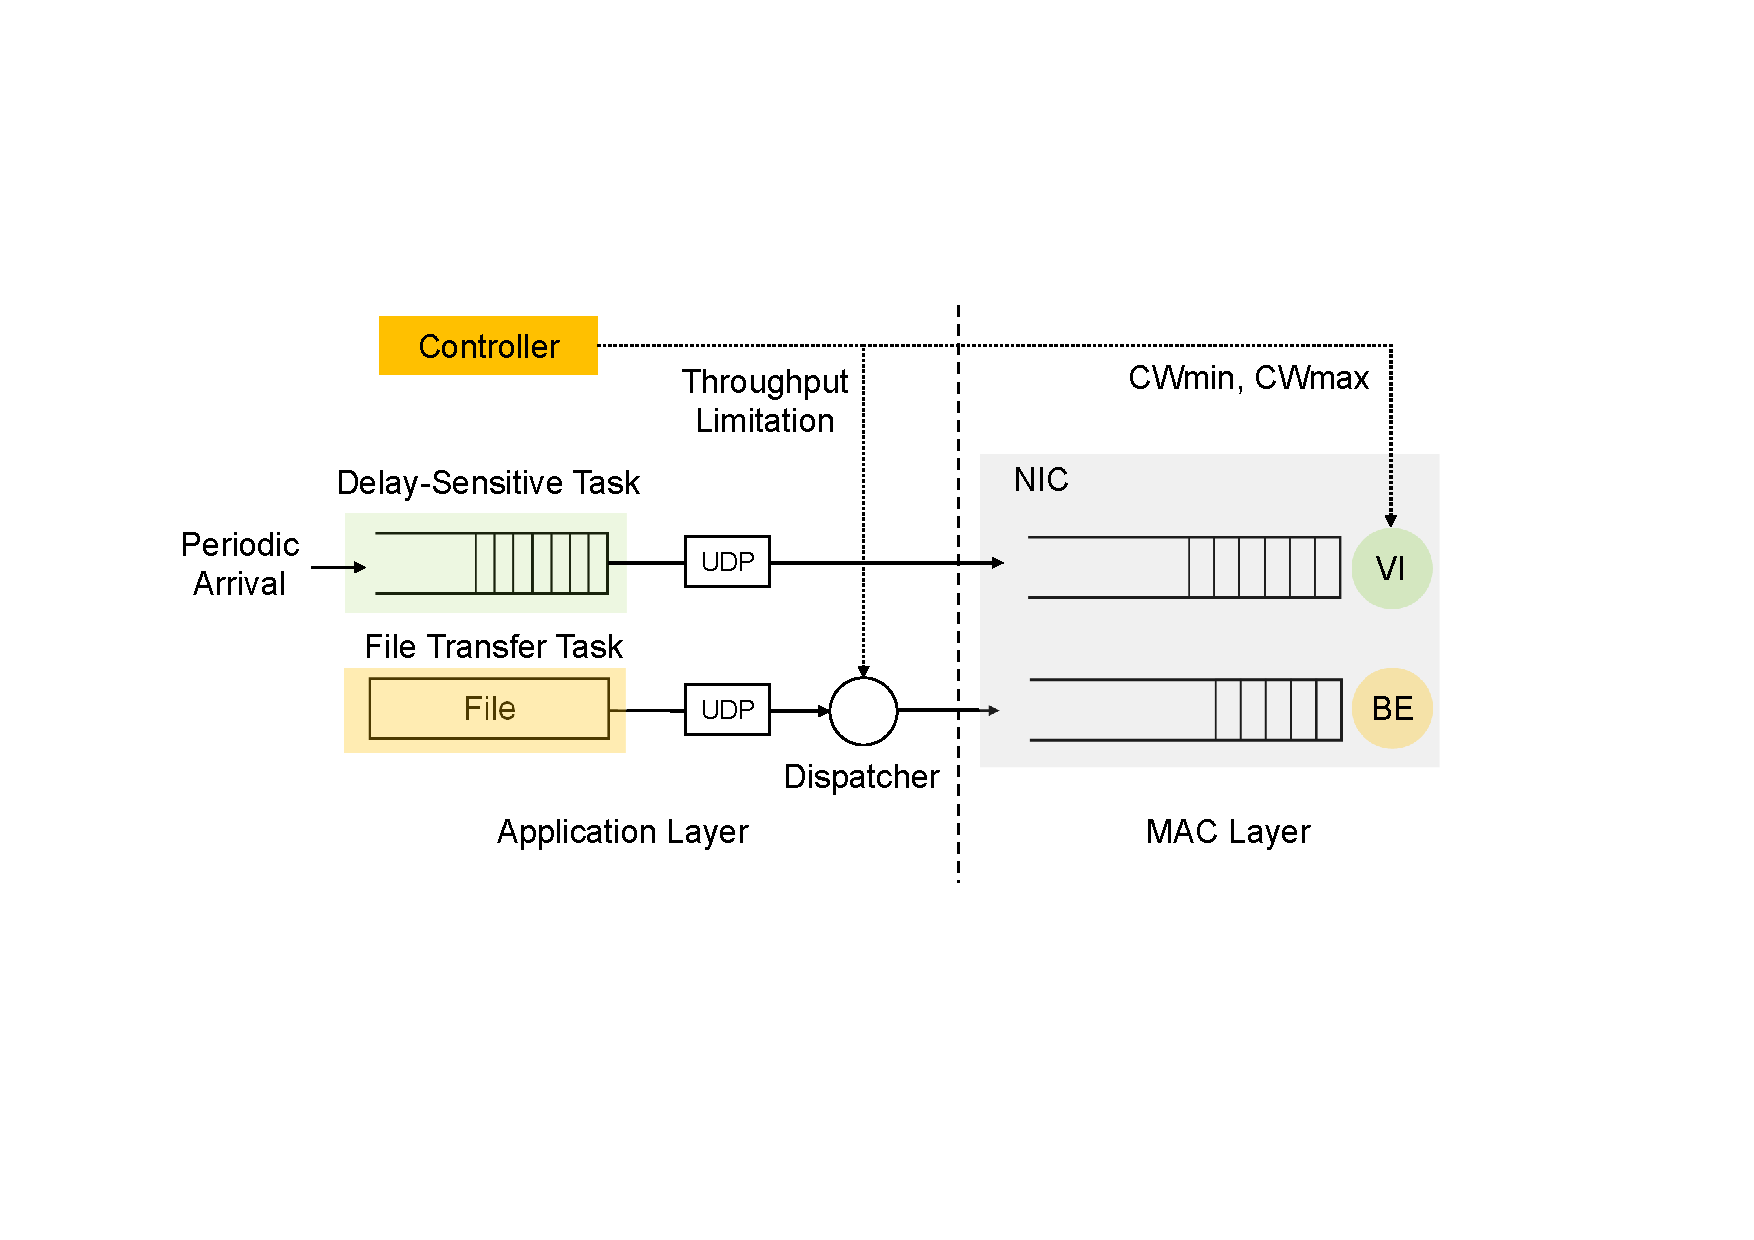
\includegraphics[width=\linewidth]{chapter3_after/MAC Queue Model 2.pdf}
    \caption{The Illustration of MAC Queue in Operating System.}
    \label{fig:MAC}
\end{figure}

\section{Problem Formulation}
\label{sec:Problem Formulation}
The proposed {\algName} system should successively make scheduling decisions for each scheduling period, which is formulated as a Markov decision process (MDP) in this section. Due to the co-channel interference, a complete description of the system state should include the traffic information of the devices in both $\devSet$ and $\devSet_I$, which is infeasible to obtain in the considered scenario. Instead, we treat the scheduling parameters and QoS observations of the past $N$ scheduling periods as the state of the current scheduling period, leading to a partially observable MDP (POMDP) with unknown state transition probabilities. Specifically, the system state, scheduling policy, and system cost are defined as follows.

\begin{definition}[System State] In the $t$-th scheduling period ($\forall t$), the system state is defined as the aggregation of the QoS observations and scheduling parameters of the past $N$ scheduling periods. Thus,
    \begin{equation}
        \state_t \define \left\{
        (\observation_{t-N},\action_{t-N}),\ldots,(\observation_{t-1},\action_{t-1})
        \right\}.
    \end{equation}
\end{definition}

\begin{definition}[Scheduling Action and Policy] Denote $\action_t$ defined in Equation (\ref{eq:action}) as the scheduling action in the $t$-th scheduling period,
\begin{equation}
    \action_t^i \define 
    \left\{ 
        b_{i,j}^m(t) | \forall j \in \linkset_i, \iterTaskThru 
    \right\} 
    \cup 
    \left\{ 
        w_{i}^{\VI}, w_{i}^{\BE} 
    \right\}.
\end{equation}
as the local scheduling action of the $i$-th device in the $t$-th scheduling period. The scheduling policy {$\Policy$} is a mapping from {state space} to {action space} as follows:
    \begin{equation}
        \Policy( \state_t ) = \action_t.
    \end{equation}
\end{definition}

Moreover, we define the system cost of the $t$-th scheduling period as
\begin{align}
    \label{eq:cost function}
    \begin{split}
        c_t(\state_t, \action_t)
        \define
         & \sum_{\iterLink} \sum_{\iterTaskRTT}
        \mathds{1}(\eleRTT(t) > \eleRTTLimit)                          \\
         & - \omega \sum_{\iterLink} \sum_{\iterTaskThru} \eleThru(t).
    \end{split}
\end{align}
where $\omega$ is a weight, $\eleRTTLimit$ is the maximum tolerable RTT of the $m$-th delay-sensitive task on the $(i,j)$-th link. The indicator function $\mathds{1}(\mathcal{E})$ is $1$ if the event $\mathcal{E}$, and $0$ otherwise.
Then, the average overall system cost is defined as the discounted summation of average system costs for all the scheduling periods, i.e.,
\begin{equation}
    \label{eq:average_cost}
    \averageCost(\Policy) = \lim_{T \rightarrow \infty} \mathbb{E}
    \bigg[
        \sum_{t = 1}^T \gamma^{t-1} c_t(\state_t, \Policy(\state_t))
        \bigg].
\end{equation}
For the elaboration convenience, it is assumed that the system has run for at least $N$ scheduling periods before the first scheduling period, such that there are sufficient QoS observations in the system state. As a result, the controller design of the {\algName} system can be formulated as
\begin{equation}
    \text{\bf Problem 1:} \ \min_{\Policy} \  \averageCost(\Policy).
\end{equation}
The Bellman's equations for the above MDP is given by
\begin{align}
    \label{eq:bellman}
    Q(\state_t, \action_t) = \mathbb{E}_{\state_{t+1}} \bigg[ c_t(\state_t, \action_t) + \gamma \min_{\action'} Q(\state_{t+1}, \action')  \bigg],
\end{align}
where $Q(\state_t, \action_t)$ is the Q-function with system state $\state_t$ and action $\action_t$. Moreover, the optimal scheduling action is given by

\begin{equation}
    \Policy^*(\state)  = \argmin\limits_{\action} Q(\state, \action).
\end{equation}

Given the past scheduling actions and QoS observations (i.e., the system state), it is still difficult to accurately predict the relation between the scheduling action and task QoS in the current scheduling period. This is because of the unknown interfering traffic. As a result, it is impossible to solve the above Bellman's equations without any trial on the network performance. In this work, we shall rely on the RL method to track the above unknown knowledge with the assistance of a preliminary observation dataset $\trainningDataSet$.

Specifically, the dataset $\trainningDataSet$ is collected from $M$ scheduling periods experiencing heterogeneous interfering traffic and link quality (e.g., the distances of links in $\linkset$ change due to mobility). Each of the scheduling periods (say the $\tau$-th one) is divided into two phases. In the first phase, a testing scheduling action $\classifyAction$ is applied, and corresponding QoS observation $\classifyObs_\tau$ is obtained; in the second phase, an arbitrary scheduling action $\trainAction_{\tau}$ according to certain criterion is applied, and another QoS observation $\trainObs_{\tau}$ is obtained. Hence,  the dataset $\trainningDataSet$  can be expressed as
\begin{equation}
    \trainningDataSet \define
    \left\{
    (\classifyObs_\tau, \classifyAction, \trainObs_{\tau}, \trainAction_{\tau})
    | \tau = \iterDataSet
    \right\}.
\end{equation}

\section{Q-Network for Online Scheduling}
\begin{figure}[!t]
   \centering
   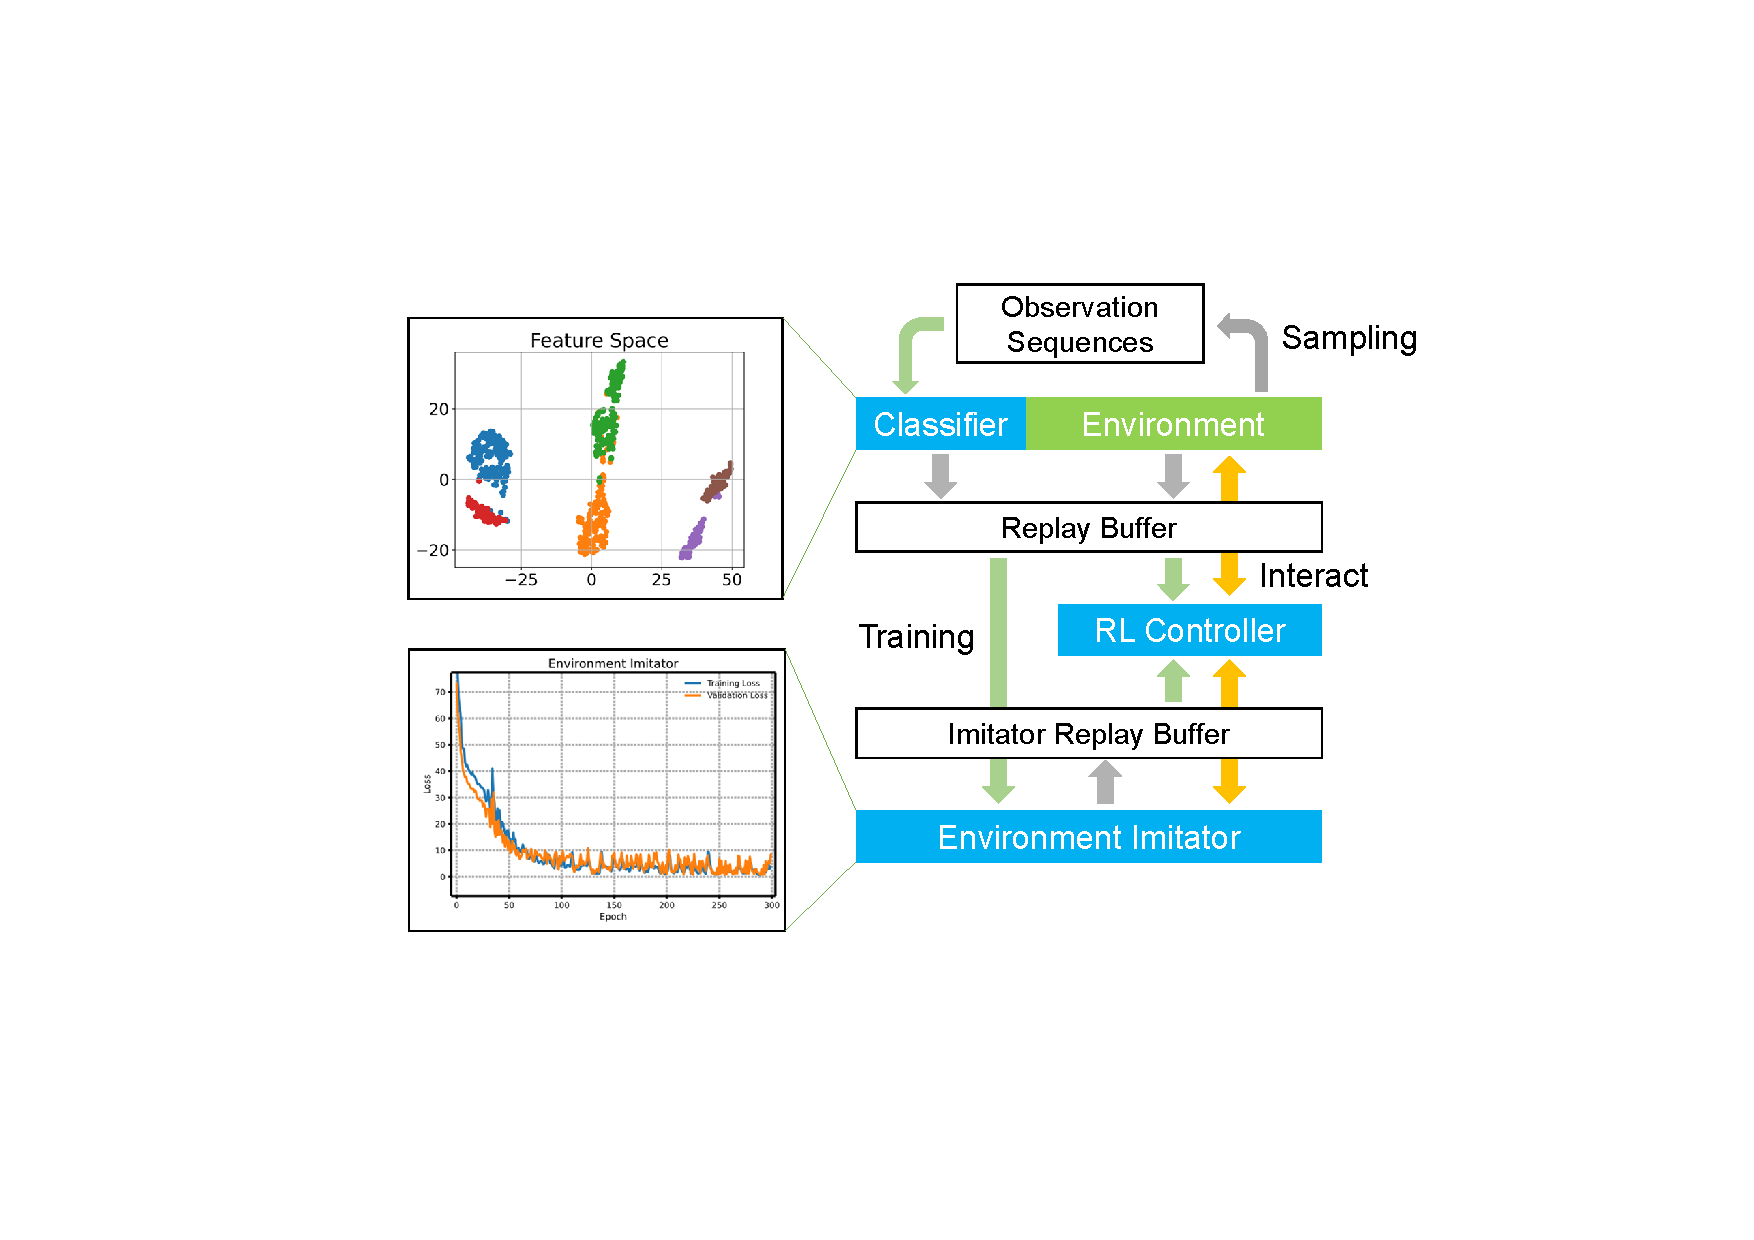
\includegraphics[width=0.9\linewidth]{chapter3_after/framework.pdf}
   \caption{The Illustration of {\algName} Online Scheduling.}
   \label{fig:framework}
\end{figure}

In this section, a novel Q-network design is proposed to approximate the Q-function defined in the previous section.
In order to accelerate the convergence of Q-network training and improve the scheduling performance, all the possible system performance of one scheduling period is divided into $K$ regions, and the inputs of the Q-network include not only the system state but also the \emph{performance region indices} of the past $N$ scheduling periods. 
Hence in this section, the offline performance region quantization based on the preliminary observation dataset $\trainningDataSet$ is introduced first, followed by the online testing of performance region index and the structure of the Q-network.

\subsection{Offline Performance Region Quantization}
\label{sec:performance Region Quantization}
The quantization of all the possible system performance is conduced based on the preliminary observation dataset $\trainningDataSet$ in an offline manner. Specifically, the QoS observations with the testing scheduling action $\classifyAction$ are extracted from the preliminary observation dataset $\trainningDataSet$ as follows:
\begin{equation}
   \classifyDataSet \define
   \left\{
   (\classifyObs_\tau, \classifyAction) | \tau = \iterDataSet
   \right\},
\end{equation}
The $K$-means classification method~\cite{macqueen1967some} is then adopted to classify the QoS observations in $\classifyDataSet$ into $K$ clusters, as illustrated in \figurename~\ref{fig:framework}. Denote the mean and variance of the observed throughputs (for the file delivery tasks) in $\classifyDataSet$ as $\avgThru$ and $\varThru^2$ respectively, the mean and variance of the RTTs (for the delay-sensitive tasks) as {$\avgRTT$ and $\varRTT^2$} respectively. Thus,
\begin{align}
   \avgThru & \define
   \frac{
      \sum_{\tau = 1}^M \sum_{\iterLink} \sum_{\iterTaskThru} \eleThruClassify(\tau)
   }{
      M \sum_{\iterLink} |\thruTS|
   },                    \\
   \avgRTT  & \define
   \frac{
      \sum_{\tau = 1}^M  \sum_{\iterLink} \sum_{\iterTaskRTT} \eleRTTClassify(\tau)
   }{
      M  \sum_{\iterLink} |\rttTS|
   },                    \\
   \varThru^2 & \define
      \frac{
         \sum_{\tau = 1}^M  \sum_{\iterLink} \sum_{\iterTaskThru}
         {\left(\eleThruClassify(\tau) - \avgThru\right)}^2
      }{
         M  \sum_{\iterLink} |\thruTS| - 1
      },                    \\
   \varRTT^2  & \define
      \frac{
         \sum_{\tau = 1}^M  \sum_{\iterLink} \sum_{\iterTaskRTT}
         {\left(\eleRTTClassify(\tau) - \avgRTT\right)}^2
      }{
         M  \sum_{\iterLink} |\rttTS| - 1
      },
\end{align}
where $\eleThruClassify$ and $\eleRTTClassify$ denote the average throughput and RTT of the $m$-th file-delivery task and delay-sensitive task on the $(i,j)$-th link in the dataset $\classifyDataSet$, respectively. Hence, the raw performance region quantization can be achieved by finding the $K$ cluster centers of the QoS observations in $\classifyDataSet$ as follows:
\begin{equation}
   \{\iterCCOpt\}  =
   \argmin
   \limits_{\iterCC} \
   \sum_{k=1}^K
   \sum_{\tau=1}^M
   \Vert \phi(\classifyObs_\tau) - \mu_k \Vert^2,
\end{equation}
where $\phi(\classifyObs_\tau)$ denotes the vectorization and normalization of the QoS observation $\classifyObs_\tau$. Specifically,
\begin{equation}
   \phi(\classifyObs_\tau) \define
   \left(
   \mathbf{r}_{\tau}^p, \mathbf{d}_{\tau}^p
   \right),
\end{equation}
where the row vector $\mathbf{r}_{\tau}^p$ vectorizes the normalized throughputs of all file delivery tasks
\begin{equation*}
   \left\{
      \frac{ \eleThruClassify(\tau) - \avgThru }{ \varThru }
      \bigg|
      \forall \iterLink, \iterTaskThru, \eleThruClassify(\tau) \in \classifyObs_\tau
   \right\},
\end{equation*}
and the row vector $\mathbf{d}_{\tau}^p$ vectorizes the normalized RTTs of all the delay-sensitive tasks
\begin{equation*}
   \left\{
      \frac{ \eleRTTClassify(\tau) - \avgRTT }{ \varRTT }
      \bigg| 
      \forall \iterLink, \iterTaskRTT, \eleRTTClassify(\tau) \in \classifyObs_\tau
   \right\}.
\end{equation*}

\subsection{Online Testing of Performance Region Index}

In the online transmission scheduling, a short testing slot can be reserved in each scheduling period, where the scheduling action $\classifyAction$ can be applied. Hence, the performance region index can be calculated according to
\begin{equation}
   \label{eq:raw performance region index}
   \rawPerRegion_t =
   \argmin\limits_{k} \
   \Vert \phi(\widehat{\observation}_t) - \mu_k^* \Vert^2,
\end{equation}
where $\widehat{\observation}_t$ is the QoS observation with the testing scheduling action $\classifyAction$ in the $t$-th scheduling period.

In the scenario where the performance region index varies slowly, the testing slot may not be applied in every scheduling period, and the performance region index of a scheduling period could follow the latest testing slot.

With the performance region quantization, we define the extended system state as follows.
\begin{definition}[Extended System State]
   Denote 
   $$
   \extendState_t \define 
   \left\{
      (\rawPerRegion_{t-N}, \observation_{t-N},\action_{t-N})
      ,\ldots,
      (\rawPerRegion_{t-1}, \observation_{t-1}, \action_{t-1})
   \right\}
   $$
   as the extended system state of the $t$-th scheduling period in the phase of online transmission scheduling, where $\rawPerRegion_{t-1}$ is the raw performance region index defined in Equation (\ref{eq:raw performance region index}).
\end{definition}

\subsection{Q-Network Structure}
\label{sec:Q-network}
\begin{figure}[!t]
   \centering
   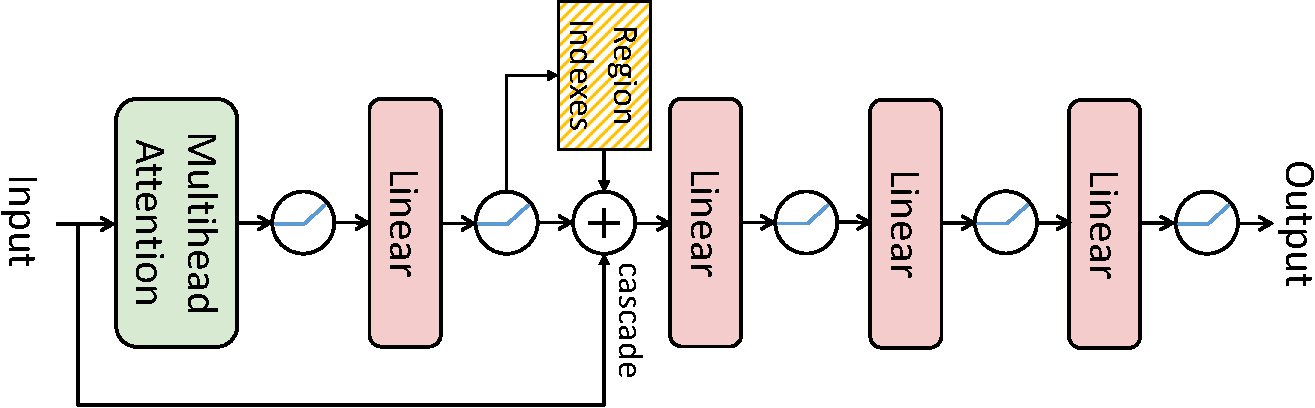
\includegraphics[width=\linewidth]{chapter3_after/Network Model 7.pdf}
   \caption{The Illustration of Novel Q-Network Design.}
   \label{fig:Network Design}
\end{figure}

The structure of the proposed Q-network is illustrated in \figurename~\ref{fig:Network Design}. Its input is the extended system state of the current scheduling period. The first part of the Q-network is a multi-head attention layer\cite{vaswani2017attention},  which is trained to refine the \emph{performance region indices} in the extended system state. The refined extended system state is then used as the input of the following three fully connected layers with $256$ nodes and ReLU activation function sequentially.

In order to address the issue of huge action space, we adopt the following linear approximation structure on the Q-function in the output of the Q-network:
\begin{equation}
   Q(\extendState, \action)
   \approx
   \sum_{{i} \in \devSet} Q^{i}(\extendState, \action^{i}),
\end{equation}
where $Q^{i}(\extendState, \action^{i})$ is referred to as the local Q-function of the ${i}$-th device. Hence, the Q-network output consists of $U$ action clusters for $U$ devices, respectively. Each action cluster provides the values of the corresponding local Q-function for all possible local actions. As a result, the optimized local action of the $i$-th device ($\forall i$) can be obtained by minimizing the local Q-function, i.e.,
\begin{equation}
   \action^{i}_t = \argmin\limits_{\action^{i}} Q^{i}(\extendState_t, \action^{i}).
\end{equation}

\section{Hybrid Q-Learning}
\label{sec:Hybrid Q-Learning}
\begin{figure*}[!t]
   \normalsize
   \begin{align}
      \label{eq: imitator loss}
      \imitatorLoss(\inetParam_k) = \frac{1}{|\trainObs_{\tau}|} \Bigg[
         \alpha
         &\sum_{\iterLink} \sum_{\iterTaskThru}
         {\left(\elePreThru(\action; \inetParam_k) - \eleThru(\tau)\right)}^2
         +
         \nonumber\\
         &\sum_{\iterLink} \sum_{\iterTaskRTTAlt}
         {\left(
            \elePreRTT(\action; \inetParam_k)
            -
            \min \left\{
            \eleRTTAlt(\tau), \beta \mathrm{D}^{n}_{i,j}
            \right\}
         \right)}^2
         \Bigg].
   \end{align}
   \begin{align}
      \label{eq:loss}
      \ctlLoss(\qnetParam_t) = \mathbb{E} \left[
         {\left( c_t\left(\state_t,\action_t\right)
         + \gamma \sum_{{i} \in \devSet}
         \min_{\action^{i'}}
         Q^{i} \left( \extendState_{t+1}, \action^{i'}; \qtnetParam_t \right)
         - \sum_{{i} \in \devSet}
         Q^{i} \left(
         \extendState_t, \action^{i}_t; \qnetParam_t
         \right)
         \right)}^2
         \right].
   \end{align}
   \hrulefill{}
\end{figure*}

The Q-network proposed in the previous section should be trained via the following two phases: the first offline training phase based on the dataset $\trainningDataSet$ and the second online tuning phase during the transmission scheduling. Both phases are elaborated in the following.


\subsection{Offline Q-learning}  

To facilitate the offline training, the performance indexes are calculated for all the scheduling periods in $\trainningDataSet$ according to Equation (\ref{eq:raw performance region index}). Denote the performance index of the $\tau$-th scheduling period in $\trainningDataSet$ as $\rawPerRegion_\tau^s$, the preliminary dataset $\trainningDataSet$ can be rewritten as
\begin{equation}
   \trainningDataSetwithRawPerInd  \define
   \left\{
   (\rawPerRegion_\tau^s, \observation_{\tau}^s, \action^s_{\tau})
   |
   \tau = \iterDataSet
   \right\}
\end{equation}
for notation convenience. Moreover, dataset $\trainningDataSetwithRawPerInd$ can be further divided into $K$ subsets as
\begin{equation}
   \trainningDataSetwithRawPerInd_k
   \define \left\{
   (k, \observation_{\tau}^s, \action^s_{\tau})
   |
   \forall \rawPerRegion_\tau^s = k
   \right\}
   \subset
   \trainningDataSetwithRawPerInd, k = \iterCCIdx.
\end{equation}

Notice that the subsets $\trainningDataSetwithRawPerInd_k$ ($k=\iterCCIdx$) may not be sufficiently large for the training of the Q-network in all the performance regions, the imitation learning method is introduced. Specifically, we first train $K$ DNN networks (namely imitators), each of which consists of $10$ fully connected layers and $256$ nodes per layer, to imitate the relation between the scheduling actions and QoS observations in the $K$ subsets, respectively. Denote the imitators as $$f(\action; \inetParam_k), k=\iterCCIdx,$$ where $\action$ is the input action, and $\inetParam_k$ represents network parameters of $k$-th performance region. The output of imitator $f(\action; \inetParam_k)$ is trained to approximate the QoS observation of the system in the $k$-th performance region with input action $\action$. Then, the Q-network can be trained via the $K$ imitators respectively.


{\bf Imitator training:} Let $\elePreThru(\action; \inetParam_k)$ and $\elePreRTT(\action; \inetParam_k)$ be the throughput and RTT of the ${m}$-th file delivery task and ${n}$-th delay-sensitive task of the $(i,j)$-th link in the output of the $k$-th imitator with input action $\action$.
The loss function of the $k$-th imitator for the training sample $(k,\trainObs_\tau, \trainAction_\tau) \in \trainningDataSetwithRawPerInd_k$, denoted as $\imitatorLoss$, is defined as Equation (\ref{eq: imitator loss}), where $r^{(m)}_{i,j}(\tau),d^{(n)}_{i,j}(\tau) \in \observation_{\tau}^s$,  $\alpha$ and $\beta$ are both weights, and the minimization is to limit the range of RTTs.

%% the imitator memory buffer
{\bf Q-network training:}  Based on the imitators, the Q-network can be trained in each performance region respectively according to the Q-learning method~\cite{mnih2015human}, where the outputs of the $k$-th imitator are treated as the QoS observations in the $k$-th performance region ($\forall k$). The loss function of the Q-learning, $\ctlLoss(\qnetParam_t)$, is defined in Equation (\ref{eq:loss}), where $Q(\cdot, \cdot; \qnetParam_{t})$ represents the Q-network updated in $t$-th scheduling period, and $\qtnetParam_t$ denotes the parameter of target network following~\cite{mnih2015human} to stabilize the training loss $\ctlLoss(\qnetParam_t)$. 

In order to efficiently explore the action space, an upper confidence bound (UCB) based exploration policy is introduced for the offline training of Q-network. Taking the Q-learning with the $k$-th imitator as the example, we first define the UCB of the action $\action^{i}$ of ${i}$-th device in the $t$-th offline scheduling period stage as
\begin{equation}
   \label{eq:UCB}
   UCB_{t}(k, \action^{i}) =
   Q_{t}^{i}(\extendState_t, \action^{i}; \qnetParam_{t})
   +
   \sqrt{\frac{4\eta\ln t}{T_{t}( k , \action^{i})}},
\end{equation}
where $T_t(k,\action^{i})$ counts the number of times the action $\action^{i}$ is taken up to the $t$-th scheduling period. The hyper-parameter $\eta$ is used to balance the exploration and exploitation.
As a result, in the $t$-th scheduling period of the offline training phase, the scheduling action is determined as follows:
\begin{equation}
   \label{eq:UCB epolicy}
   \action_t^{i} = \begin{cases}
      \argmin UCB_{t}(k, \action^{i}) & \text{with probability } 1 - \epsilon_t, \\
      \action^{i} \sim \uniformDis(\actionSpace^{i}) & \text{with probability } \epsilon_t,
   \end{cases}
\end{equation}
where $\uniformDis(\actionSpace^{i})$ is the uniform distribution over action space $\actionSpace^{i}$ of ${i}$-th device and exploration rate $\epsilon_t$ should satisfy the limit condition $\lim_{t \to \infty} \epsilon_t = 0$.

\subsection{Online Q-learning} 
The Q-network after the offline training is adopted in online scheduling. Meanwhile, the online training with the same loss function as in Equation (\ref{eq:loss}) could be applied to further improve the performance of the proposed {\algName} system. Specifically, in the $t$-th scheduling period of online training, the scheduling action of the ${i}$-th device, denoted as $\action_t^i$, is determined by the $\epsilon$-greedy policy as follows:
\begin{equation}
   \label{eq:online epolicy}
   \action_t^{i} = \begin{cases}
      \argmin Q^{i}(\extendState_t, \action^{i}; \netParam_{t}) & \text{with probability } 1 - \epsilon_t, \\
      \action^{i} \sim \uniformDis(\actionSpace^{i})            & \text{with probability } \epsilon_t,
   \end{cases}
\end{equation}
where $\epsilon_t$ and $\uniformDis(\actionSpace^{i})$ are defined in Equation (\ref{eq:UCB epolicy}).

\section{Experiments}
\label{sec:chapter3_after-testbed}

\begin{figure}[!t]
    \centering
    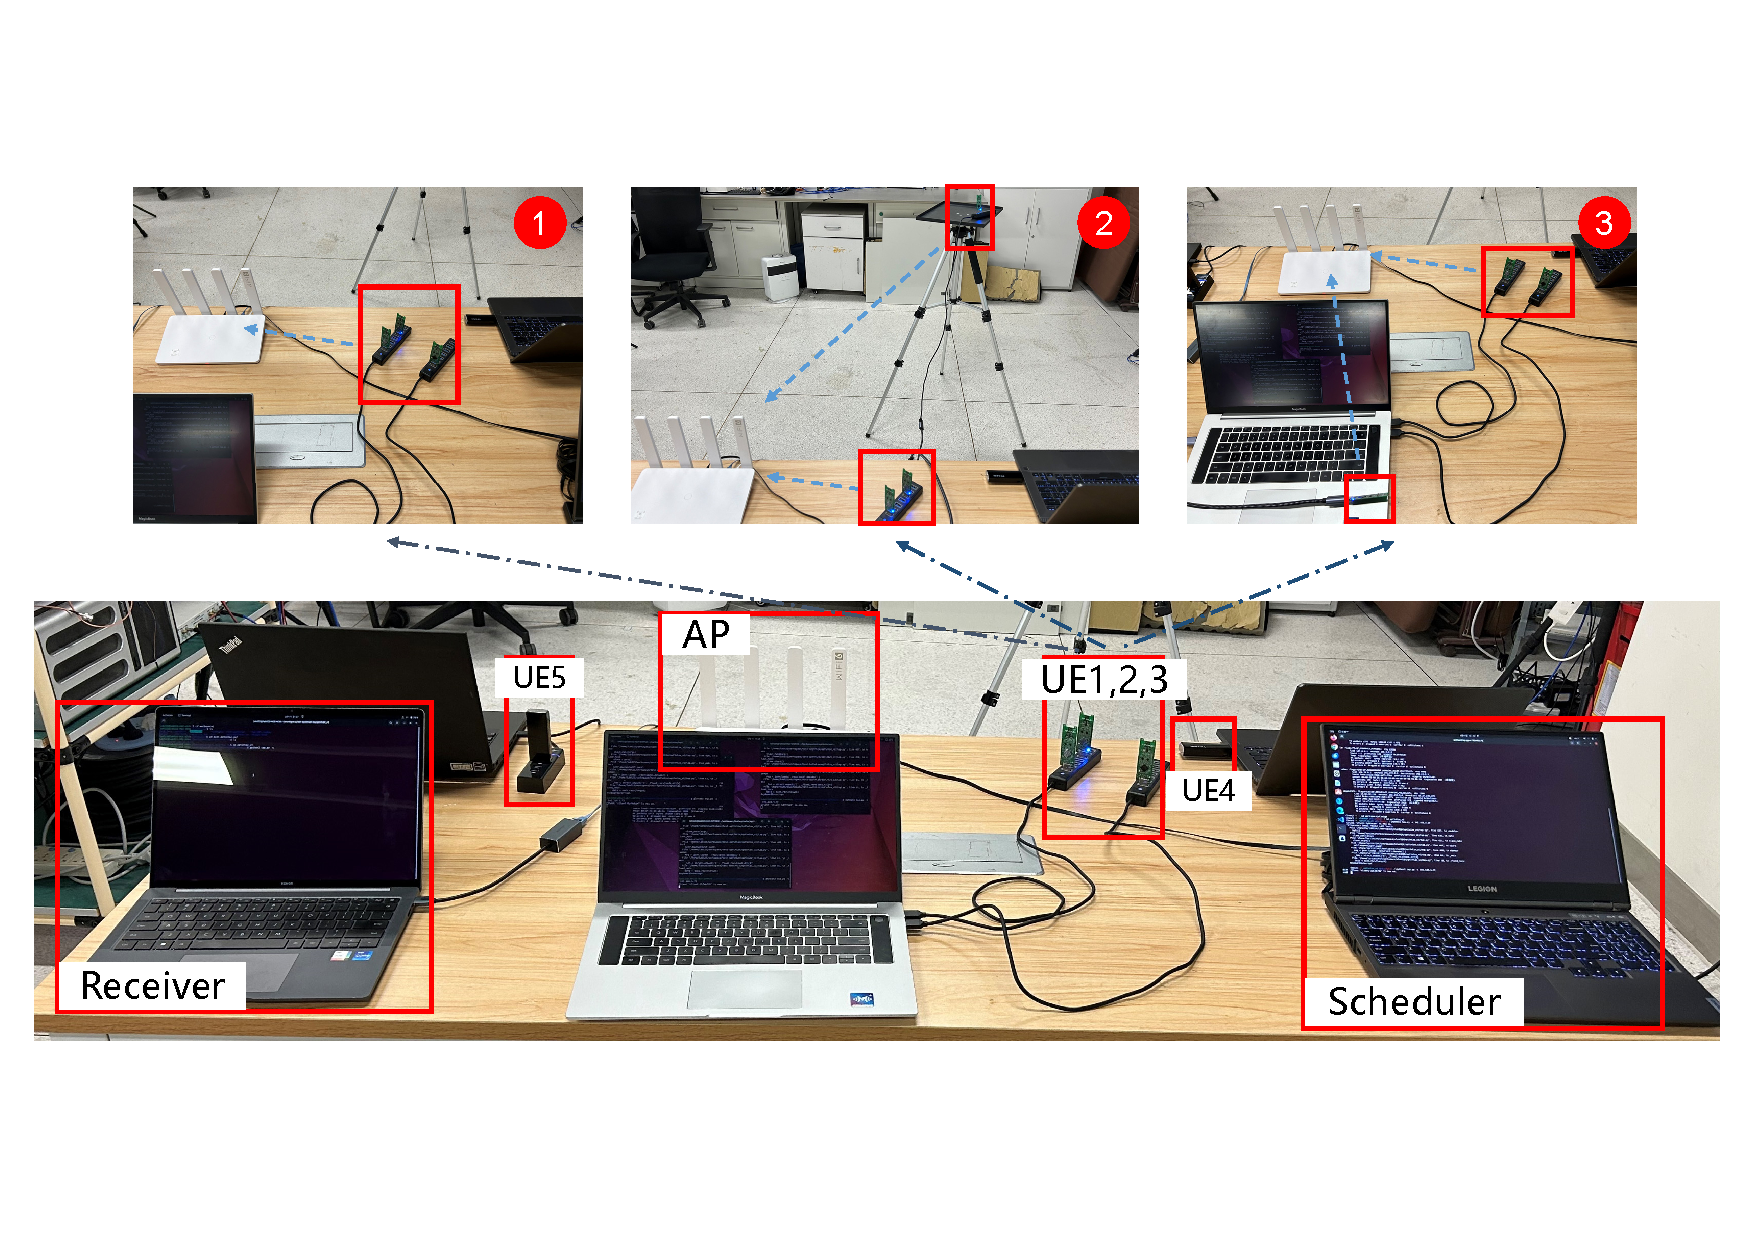
\includegraphics[width=1\linewidth]{chapter3_after/testbed-4.pdf}
    \caption{The testbed for experiments: below, the transmission scenario; above, $3$ evaluation examples.}
    \label{fig:Testbed Setup}
\end{figure}

As illustrated in \figurename~\ref{fig:Testbed Setup}, the proposed {\algName} framework is implemented in a Wi-Fi network with one HONOR XD30 AP and $3$ UEs each equipped with a TP-Link TL-WDN62000 USB Wi-Fi adapter in the experiment. 
Denote the AP as $u_0$ and the three UEs as $u_1, u_2, u_3$, respectively. 
% Reference: https://www.tp-link.com.cn/product_364.html?v=specification
The network is working on the 5GHz Wi-Fi band following the IEEE802.11ac specification.
The real-time controller is implemented in a laptop with Intel Core i7-8750H CPU and Ubuntu 20.04 operating system. % chktex 8
An Ethernet connection with a maximum data rate of $1$ Gbps is employed to facilitate communication between the controller and the AP.\@ 
Moreover, we rely on the Linux module \textit{wlspos\_hack}~\cite{lasso-sustech_wlsops-hack_2023} to adapt the CW sizes of TL-WDN62000 adapters in real-time from user space. 
Hence, the controller can collect the QoS observations from the three UEs and notify the scheduling actions via Wi-Fi, such that the UEs' transmission scheduling can be adjusted accordingly.

Both file delivery tasks and delay-sensitive tasks are tested in the experiment. The former tasks with a sufficient backlog are transmitted with the BE priority. The latter tasks, consisting of two types, are delivered with the VI priority. The data rates of type I and II delay-sensitive tasks are $\lambda_1 = 50$Mbps and $\lambda_2 = 25$Mbps, respectively. The packet arrival intervals of the two types are both  $16$ ms. Moreover, the maximum tolerable RTTs are $16$ms and $28$ms, respectively. The universal set of communication tasks tested in the experiment includes:
\begin{itemize}
    \item A delay-sensitive task with arrival data rate $\lambda_1$ (Task 1) and a file delivery task (Task 2) on the $(u_1,u_0)$-th link;
    \item A delay-sensitive task with arrival data rate $\lambda_2$ (Task 3) on the $(u_2,u_0)$-th link;
    \item A delay-sensitive task with arrival data rate $\lambda_2$ (Task 4) on the $(u_3,u_0)$-th link.
\end{itemize}
The quality of the $(u_1,u_0)$-th, $(u_2,u_0)$-th and $(u_3,u_0)$-th links depends on their distances and the propagation environment, which could be changed in the experiment. 

In the experiment, the duration of scheduling period is 1 seconds, the CW size takes values from $\{2^{i} \mid i = 0,1,2,\dots,10\}$ and throughput limitation takes values from $\{ \frac{i}{20} r_{i,j}^{({m},\max)} \mid i =0,1,2,\dots,20\}$, where $r_{i,j}^{({m},\max)}$ = 600 Mbps. Moreover, in addition to the background interference, the interfering traffic between two interfering UEs, denoted as $u_4$ and $u_5$, 
is also generated with random data rate and BE priority in the same channel. 

The preliminary observation dataset $\trainningDataSet$ are collected from the following three different traffic patterns: (1) Tasks 1 and 2 are activated; (2) Tasks 1, 2, and 3 are activated; and (3) Tasks 1, 2, 3 and 4 are activated. In all the traffic patterns, the communication distances of the links are altered to exploit the diversity of link rates. In the collection of  $\trainningDataSet$, the testing scheduling action $\action^p$ is first applied in the first half of the scheduling period, where the CW size and throughput limitation are $7$ and $300$ Mbps respectively. Then, a randomized action is applied in the second half. QoS observations of both actions are collected in each scheduling period. 

To demonstrate the performance gain, the proposed framework is compared with two baselines. The first baseline relies on the conventional 802.11 EDCA protocol. The second baseline only adapts the throughput limitation of file delivery tasks via the proposed framework, the control of the CW size follows the conventional 802.11 EDCA protocol.

\subsection{Imitator and Q-Network Training}

\begin{figure}[!t]
    \centering
    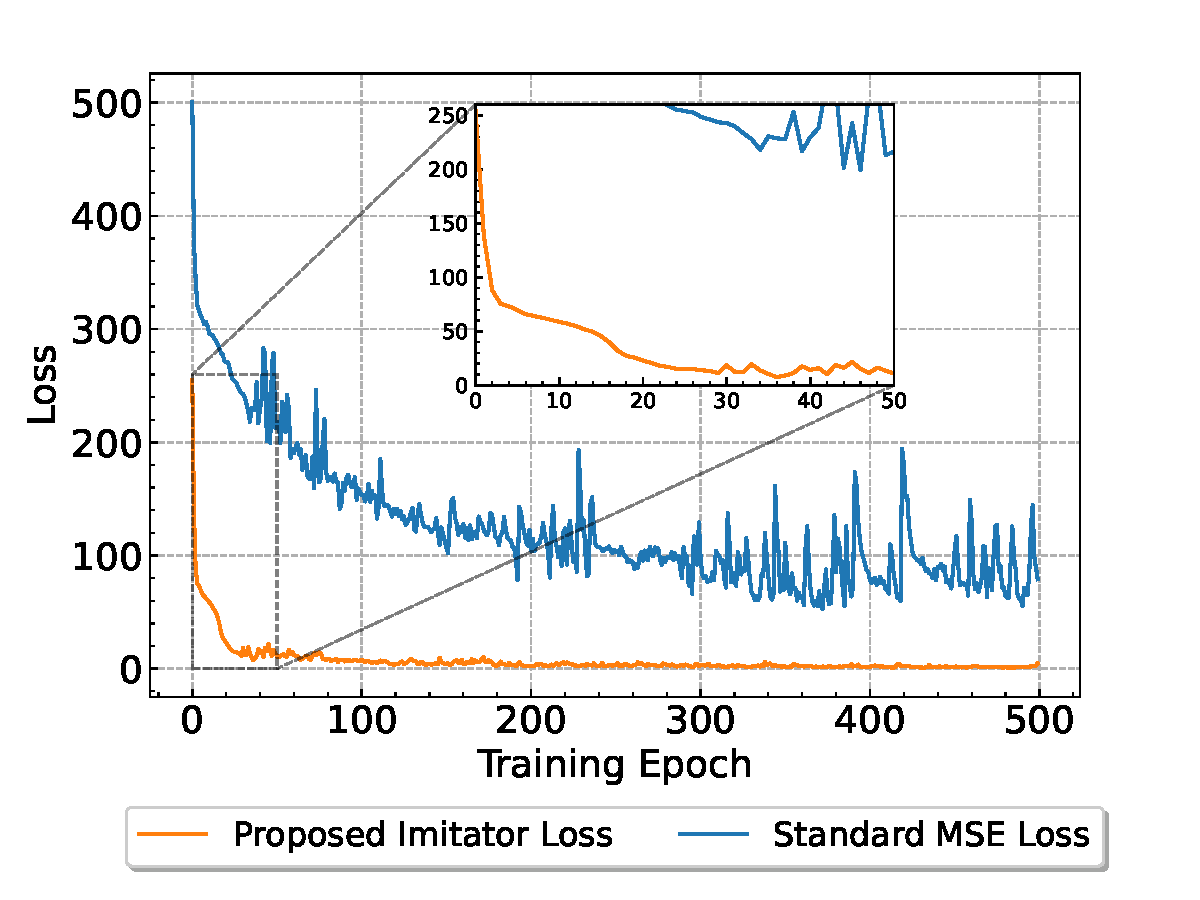
\includegraphics[width=\linewidth]{chapter3_after/loss compare-7.pdf}
    \caption{Comparing imitator training loss: proposed imitator loss function (\ref{eq: imitator loss}) versus standard MSE loss.}
    \label{fig:imitator training loss} % chktex 24
\end{figure}
\begin{figure}[!t]
    \centering
    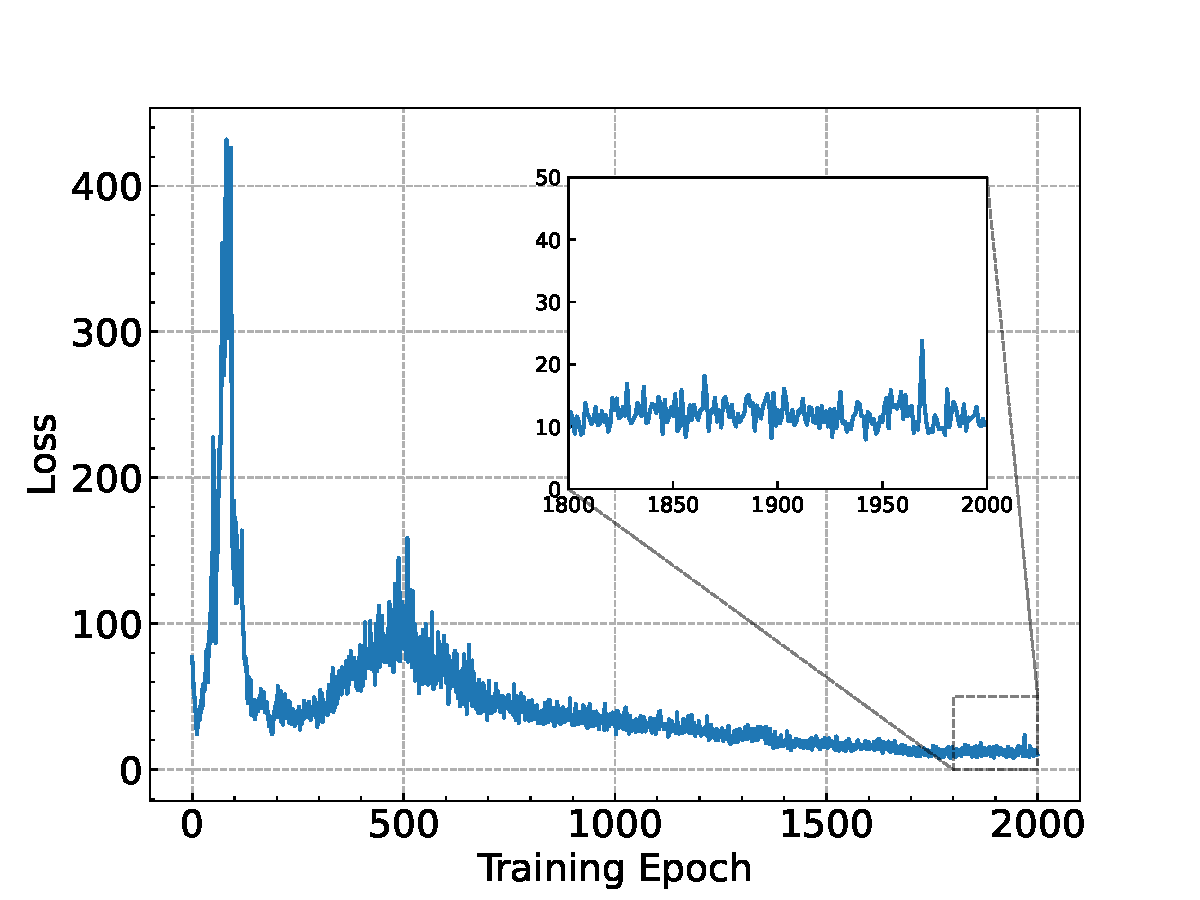
\includegraphics[width=\linewidth]{chapter3_after/rl_loss_2.pdf}
    \caption{The scheduler training loss following Equation (\ref{eq:loss}).}
    \label{fig:scheduler training loss} % chktex 24
\end{figure}
\begin{figure*}[!t]
    \centering
    \begin{minipage}[b]{0.32\linewidth}
        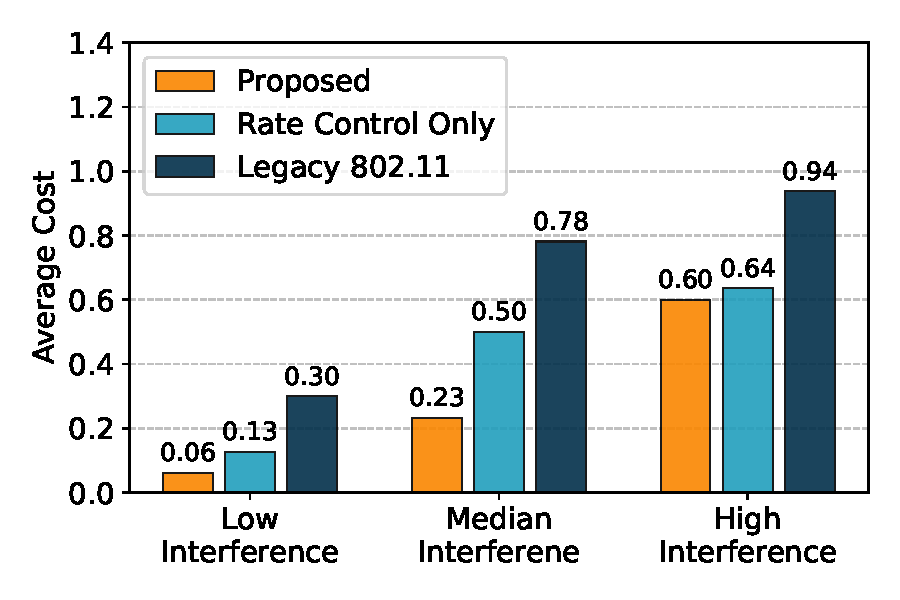
\includegraphics[width=\linewidth]{chapter3_after/Scenario 1-Average Cost 5.pdf}
        \caption*{(a) Scenario 1}
    \end{minipage}
    \begin{minipage}[b]{0.32\linewidth}
        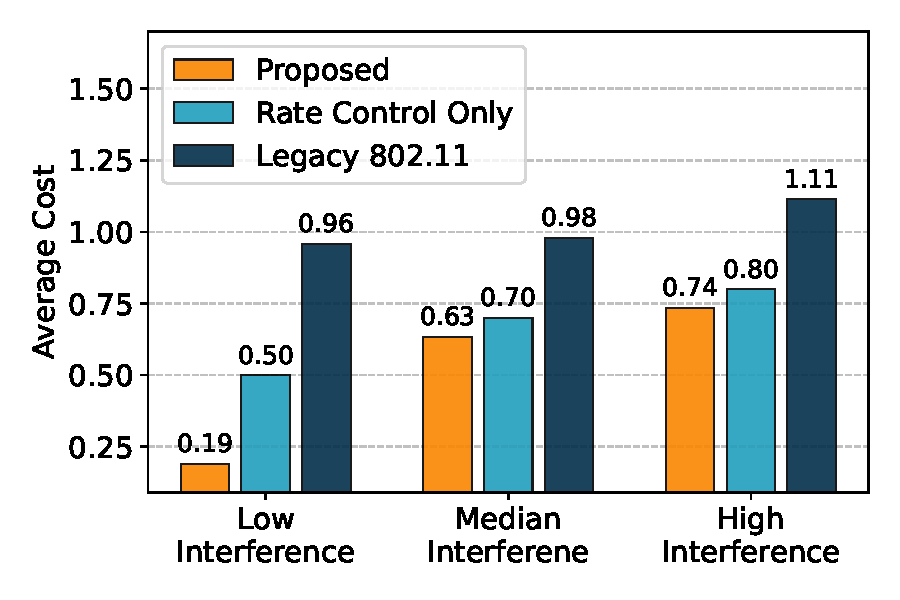
\includegraphics[width=\linewidth]{chapter3_after/Scenario 2-Average Cost 5.pdf}
        \caption*{(b) Scenario 2}
    \end{minipage}
    \begin{minipage}[b]{0.32\linewidth}
        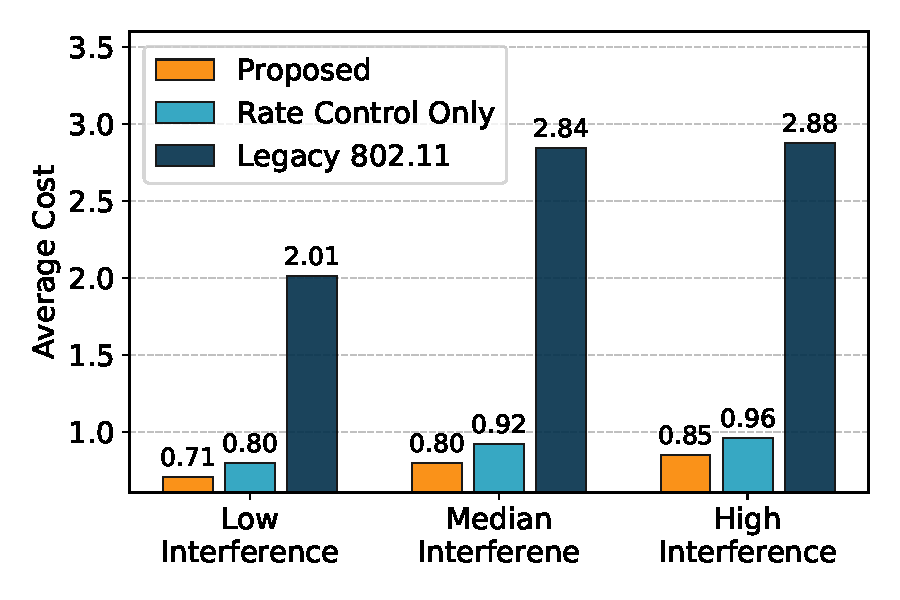
\includegraphics[width=\linewidth]{chapter3_after/Scenario 3-Average Cost 5.pdf}
        \caption*{(c) Scenario 3}
    \end{minipage} \\
    \begin{minipage}[b]{0.32\linewidth}
        \centering
        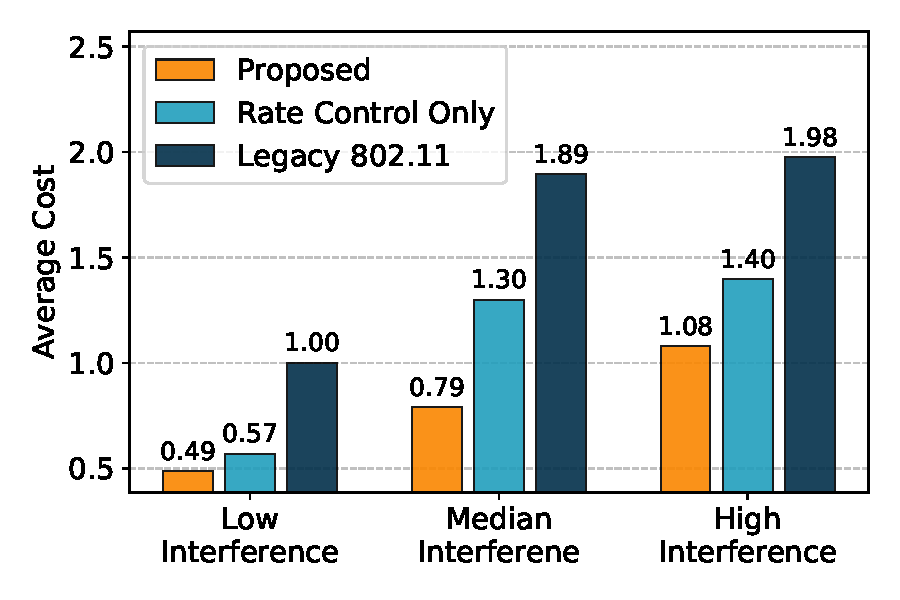
\includegraphics[width = 1\linewidth]{chapter3_after/Scenario 4-Average Cost 5.pdf}
        \caption*{(d) Scenario 4}
    \end{minipage}
    \begin{minipage}[b]{0.32\linewidth}
        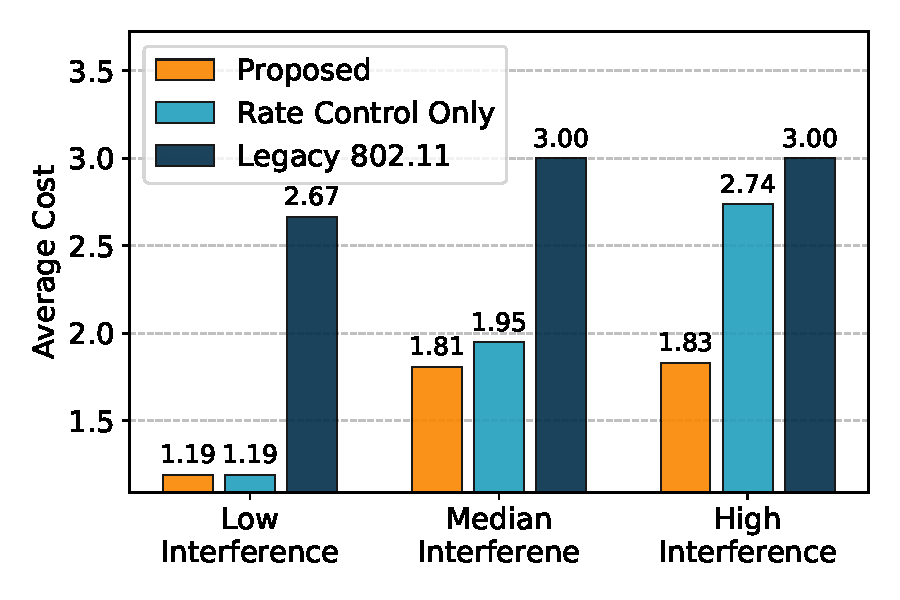
\includegraphics[width = 1\linewidth]{chapter3_after/Scenario 5-Average Cost 5.pdf}
        \caption*{(e) Scenario 5}
    \end{minipage}
    \caption{Comparing average costs across proposed algorithm, rate control only, and legacy 802.11 for evaluation scenarios from 1 to 5.}
    \label{fig:Average cost comparison of proposed algorithm in Scenario 1, 2, 3, 4 and 5.} % chktex 24
\end{figure*}


Based on dataset $\mathscr{S}^s$, the performance of the three traffic patterns are quantized into 3, 6 and 6 regions, respectively. Then, $15$ QoS imitators are trained with the tools of \textit{CUDA}\cite{cuda} and \textit{pytorch}\cite{NEURIPS2019_9015} according to Section~\ref{sec:Hybrid Q-Learning} with $\alpha=1$, $\beta=3$. Given the trained QoS imitators, the Q-network is further trained as elaborated in Section~\ref{sec:Hybrid Q-Learning} with $\omega=1/{r}^{(m,\max)}_{i,j}$.

The convergence of imitator and offline Q-network training is illustrated in \figurename~\ref{fig:imitator training loss} and \figurename~\ref{fig:scheduler training loss}, respectively. Specifically, the training loss of the imitator for the traffic scenario $3$ is illustrated in \figurename~\ref{fig:imitator training loss}, where the convergence performance of the proposed loss function in Equation (\ref{eq: imitator loss}) is compared with that of the standard MSE loss function. The proposed loss function is observed to ensure a significantly faster convergence rate. Specifically, 200 epochs are requested for convergence with the standard MSE loss function, while this number is reduced to 30 epochs with the proposed loss function.


\subsection{Performance Evaluation}
\label{Evaluation_Scenarios} % chktex 24
\begin{table}[!t]
    \centering
    \begin{tabular}{c|c|c|c} % chktex 44
    \specialrule{.1em}{.05em}{.05em} 
    Scenario  
    & 
    \begin{tabular}[c]{@{}c@{}}Traffic\\ Pattern\end{tabular}      
    & 
    Link                          
    & 
    \begin{tabular}[c]{@{}c@{}}Maximum Link Rate\\(Mbps)\end{tabular}  
    \\ 
    \hline % chktex 44
    \hline % chktex 44
    6   & 3    & $(u_3, u_0)$                           & 476       \\ \hline         % chktex 44
    7   & 3    & $(u_2, u_0)$                           & 424       \\ \hline         % chktex 44
    8   & 2    & $(u_2, u_0)$,$(u_3, u_0)$        & 400, 346  \\ \hline         % chktex 44
    9   & 3    & $(u_2, u_0)$,$(u_3, u_0)$        & 400, 346  \\ \hline         % chktex 44
    10  & 2    & $(u_1, u_0)$                           & 459       \\ \hline         % chktex 44
    11  & 3    & $(u_1, u_0)$                           & 459       \\ \hline \hline  % chktex 44
    \end{tabular}
    \caption{The maximum link rates of test scenarios from 1 to 6.\label{tab:Test Scenario}}
\end{table}

In this section, the performance of the proposed scheduling framework is showcased through evaluation across 11 distinct scenarios, with $3$ of them are listed in \figurename~\ref{fig:Testbed Setup}. These scenarios are subdivided into groups of 5 and 6 to assess both the performance and generalization capability of the proposed algorithm, respectively.

% Evaluate the performance of the proposed algorithm
In evaluating the algorithm performance, the first $3$ scenarios follow the traffic patterns where the maximum link rate of each link is $563$, $499$, and $572$ Mbps, respectively. 
Moreover, scenarios 4 and 5 follow the traffic patterns 2 and 3 with the maximum link rate reduction to $370$ Mbps of $(u_2, u_0)$.
Specifically, each traffic pattern is engaged with $3$ individual interference levels, namely \textit{Low Interference}, \textit{Medium Interference} and \textit{High Interference}, where the interference traffic rate is $0$, $50$ and $100$ Mbps, respectively. 

% Results
The average cost of the proposed algorithm, rate control only, and legacy 802.11 are compared in \figurename~\ref{fig:Average cost comparison of proposed algorithm in Scenario 1, 2, 3, 4 and 5.}. From the comparisons, the proposed algorithm outperforms both the rate control only algorithm and the legacy 802.11 mechanism in all five scenarios, which demonstrates the effectiveness of the proposed algorithm in the scheduling of combinations of delay-sensitive tasks and file delivery tasks.

\begin{figure}[!t]
    \centering
    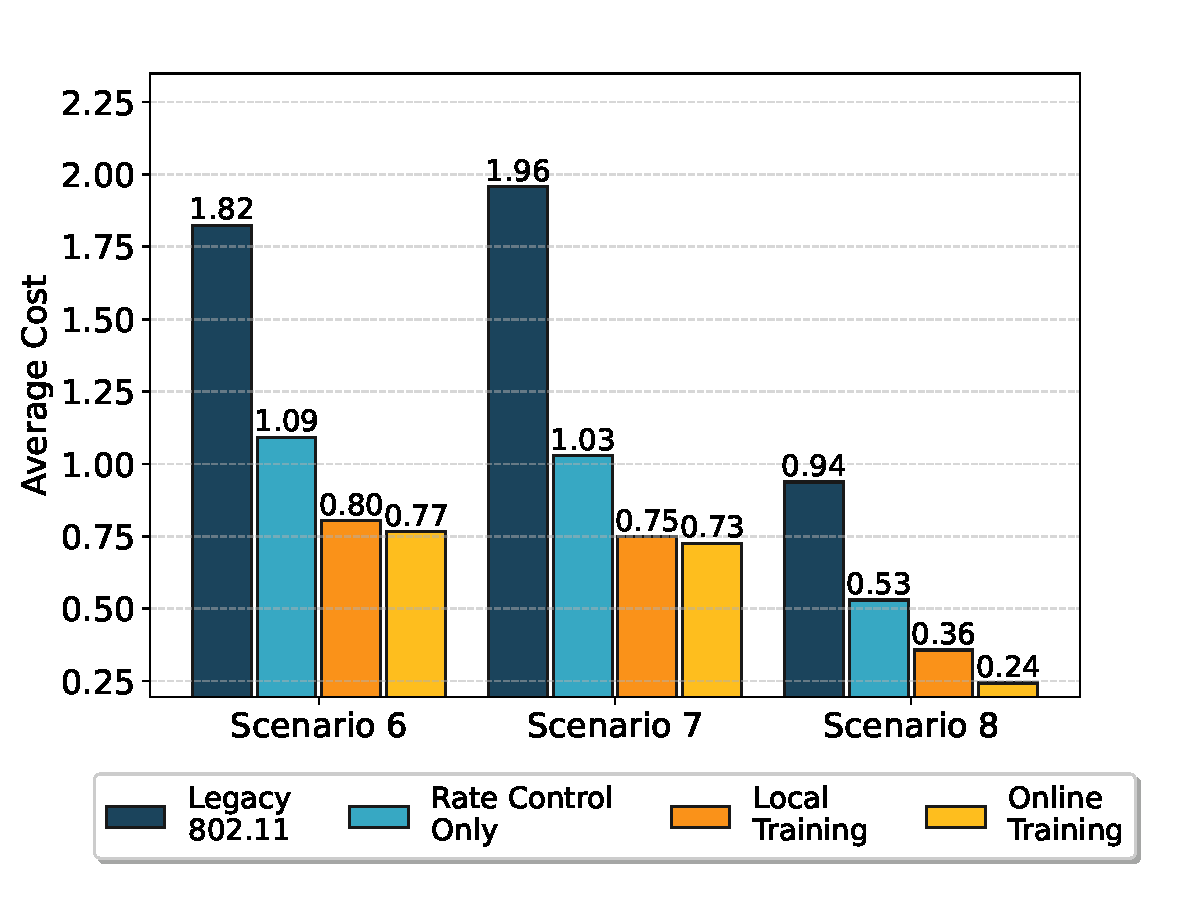
\includegraphics[width=\linewidth]{chapter3_after/test-case1-3.pdf} % chktex 8
    \caption{Comparing average costs across legacy 802.11, rate control only, Q-network trained offline (Local Training), and Q-network trained online (Online Training) for scenarios 6, 7, and 8.\label{fig:Test-changing interference-cost for test scenario 6, 7 and 8.}}
\end{figure}

\begin{figure}[!t]
    \centering
    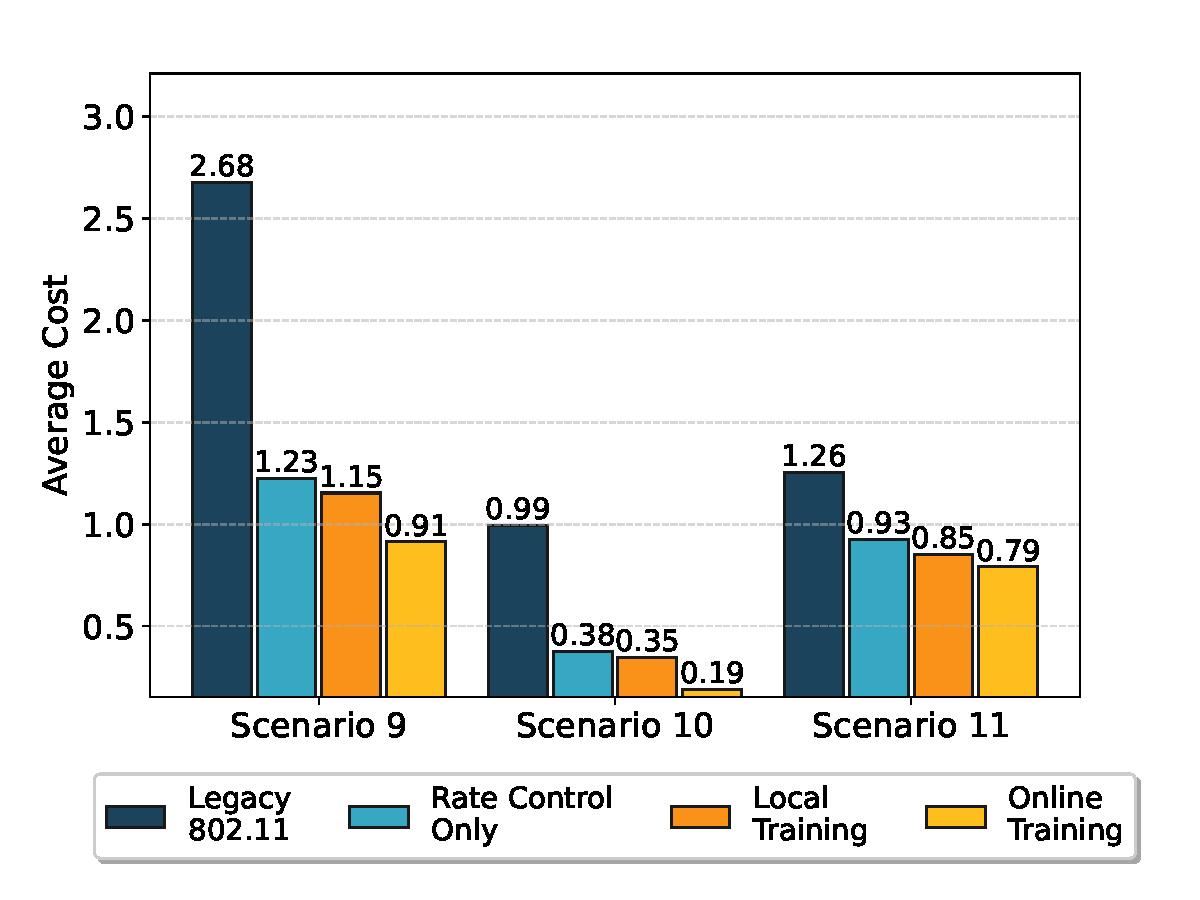
\includegraphics[width=\linewidth]{chapter3_after/test-case2-3.pdf} % chktex 8
    \caption{Comparing average costs across legacy 802.11, rate control only, Q-network trained offline (Local Training), and Q-network trained online (Online Training) for scenarios 9, 10, and 11.\label{fig:Test-changing interference-cost for test scenario 9, 10 and 11.}}
\end{figure}

%% Evaluate generation ability
In evaluating the generalization ability of the proposed algorithm, the proposed algorithm is further evaluated in $6$ test scenarios, where distance of link $(u_1,u_0)$, $(u_2,u_0)$ and $(u_3,u_0)$ are modified inducing a modified maximum link rate as Table~\ref{tab:Test Scenario}. During the evaluation, the locally trained scheduler is first used to control the transmission, which results in the \textit{Local Training} column. After that, the scheduler is further trained in an online manner following Equation (\ref{eq:online epolicy}), which results in the \textit{Online Training} column.

% Results
The average costs of the proposed algorithm and baselines in \figurename~\ref{fig:Test-changing interference-cost for test scenario 6, 7 and 8.} and \figurename~\ref{fig:Test-changing interference-cost for test scenario 9, 10 and 11.} showcase that localized training network is effective in scheduling under the unseen network condition, indicating a good generalization capability of the local trained network. 
Moreover, the scheduling under the online trained network results in an improved system performance, demonstrating the effectiveness of the online training mechanism.

\section{Summary}
\label{sec:chapter3_after-conclusion}
In this chapter, we consider the problem of optimizing the Quality of Service (QoS) of application-layer traffic in IEEE 802.11 networks. We propose a deep reinforcement learning-based channel access framework, {\algName}, which dynamically adjusts the Enhanced Distributed Channel Access (EDCA) parameters and throttles the throughput-hungry file streams to optimize the QoS of application-layer traffic.
We validate our proposed algorithm through commercial-off-the-shelf (COTS) hardware testbed.
Our results show that {\algName} can achieve a Pareto optimal of throughput and Round-Trip Time (RTT) for complex application-layer traffic under various network conditions.
% }
